\subsection{The NIC Datapath}
\label{ssec:nic-datapath}
The NIC datapath processes packets as they enter and leave the network.
Figure~\ref{fig:nanoPU} shows a high-level block diagram of the NIC packet-processing datapath.

The centerpiece of the NIC datapath is an event-driven PISA pipeline~\cite{event-driven-pisa}. 
The original PISA architecture, proposed in the RMT chip~\cite{RMT} and later used by Tofino~\cite{tofino}, is designed for mostly-stateless match-action processing of packet headers; for example for lookups, encapsulation, tunnels and telemetry.
Basic PISA only supports one type of event: the arrival of new packets. 
{\em Event-driven} PISA enhances the basic model to support other event types, such as packet drops, timers and state-dependent events. 
Section~\ref{ssec:nic-transport} describes how an event-driven PISA pipeline can directly support transport protocols in hardware, thus offloading per-packet processing from the CPU. 

The PISA pipeline also performs protocol processing: depending on the loaded P4~\cite{P4} program, it might add and remove Ethernet, IP, VXLAN, GRE, INT~\cite{INT} and transport headers. 
We also program it to add or remove a small per-context header containing the source IP address, a context ID, and message length~\Cref{fig:app-headers}.

\begin{figure}
 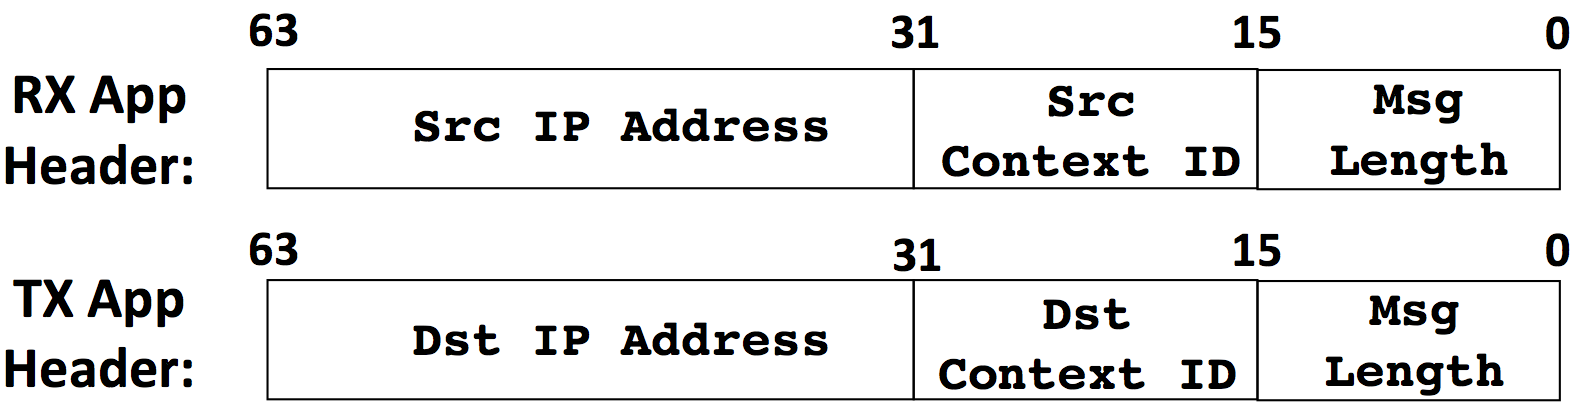
\includegraphics[width=\linewidth]{./figures/app-headers}
 \caption{Application header formats used in the NIC-Core interface.}
 \label{fig:app-headers}
\end{figure}

As others have noted, a P4-programmable PISA pipeline can also be used to accelerate some applications by offloading processing from the CPU (\eg, memory and disk caches~\cite{netcache}, load-balancers~\cite{silkroad}, consensus protocols~\cite{netchain} and firewalls~\cite{p4-firewall}). 
The L-NIC paper~\cite{lnic} describes how a PISA pipeline can accelerate nanoservices to search the Othello state-space.
